\cotefile{29}
\scanpage{95}
% archive sheet number: 94
tera donc du e) dans le

\uline{Corollaire} 3.2. Soi\inserted{en}t $S$ un préschéma non vide, $u:M'\quad M$ un homomorphisme de groupes commutatifs ordinaires, $u':G\quad G'$ l'homomorphisme transposé . Alors :

a) Pour que $u$ soit un monomorphisme, il f et s que $u'$ soit fidèlement plat.

b) Pour que $u$ soit un épimorphisme, il f et s que $u'$ soit un monomorphisme (et alors $u'$ est même une immersion fermée).

Pour prouver a), on note que si $u$ est un monomorphisme, alors
$\underline{\mathrm O}_S(M)$ est un Module \deleted{\unsure{libre sur|libre}} \inserted{sur} $\underline{\mathrm O}_S(M')$, \deleted{tout système \unsure{de} représentants}
admettant une base non vide (savoir, le système de sections défini par
n'importe quel système de représentants dans $M$ modulo $M'$), à fortiori
il est fidèlement plat. Réciproquement, s'il en est ainsi, alors $\underline{\mathrm O}_S(M')\quad
\underline{\mathrm O}_S(M)$ est injectif, ce qui (pour $S\ne\varnothing$) implique que $u:M'\quad M$ est
injectif.

Pour prouver b), on note que si $u$ est un épimorphisme, alors
$\underline{\mathrm O}_S(M')\quad\underline{\unsure{\mathrm O|\mathrm C}}_S(M)$ est surjectif, donc $u'$ est une immersion fermée et à
fortiori un monomorphisme. Inversement, s'il en est ainsi, alors $\operatorname{Ker} u'={}$ groupe unité , or \deleted{posant} posant $M''=\operatorname{Coker}u$, on a vu que
$\operatorname{Ker}u'\quad D_S(M'')$, donc par 2.1. d) on a $M''=0$ donc $u$ est un épimorphisme.

On conclut de 3.1. de la façon habituelle:

\uline{\unsure{Corollaire|Copollaire}} 3,3, Soit $M'\overset{u}{\quad} M\overset{v}{\quad} M''$ une suite exacte de groupes
commutatifs ordinaires, considérons la suite transposée
\[
G''\overset{v'}{\quad} G\overset{u'}{\quad}G'\quad .
\]
Alors $v'$ induit un morphisme fidèlement plat et quasi-compact de $G''$
dans $\operatorname{Ker}u'$, et ce dernier est un groupe diagonalisable.
\scanpage{96}
\mspage{5}
% archive sheet number: 95
on ait $n\gamma=\sum_{0}^{\unsure{n|u}} c_i\beta_i$

On utilise maintenant le théorème de Kummer pour $\mathfrak X/\unsure{\underline D_0|D}$ pour trouver
un \unsure{revêtement} de $\mathfrak X/\underline D_0$ qui ait comme
groupe \deleted{\unsure{d'inertie}} de Galois $J_0$\inserted{$\simeq\mu_n$}, et p.r son
groupe d'inertie en $X_0$ \ldots..

\margin{$\deleted{\unsure{B}}\beta^0=n\gamma+\sum_1^r c_i\beta^{i}$\\
$\unsure{\mathscr L|\mathscr D|\mathcal J}\simeq K^{\otimes n}$}
\diagram{\begin{tikzcd}[ampersand replacement=\&,column sep=small]
\pi_2^t(X_0/D'_0,\bar\xi_0)\arrow[r]\arrow[r,no head,start anchor=south,end anchor=south,to path={-- ++(0,-.28) -| (\tikztotarget)}] \& \mu^\infty_{X_0,t}(\bar\xi_0)\arrow[r] \& \pi_1^t(\mathfrak X/D,\bar\xi_1)\arrow[r] \& \pi_1^t(X_0/D'_0,\bar\xi_0)\arrow[r]\arrow[ll,bend right=28,start anchor=north,end anchor=north east] \& 0
\end{tikzcd}}

$\pi_1^t(\mathfrak X/D,\bar\xi_1)$ comme extension de $\pi_1^t(X_0/D'_0,\bar\xi_0)$
est connu \unsure{entièrement} en termes de
$X_0/D'_0$ et de la classe $\alpha\in H^2(X_0\deleted{\unsure{-D'_0|-D_0}},\mu^\infty_{X_0,\mathrm{tame}})$
[self-intersection de $X_0$ dans $\mathfrak X$] \ldots.

\uline{Exemple I} $X_0$ courbe algébrique \inserted{lisse} sur $k$ \unsure{alg.|sép.} clos.

Alors $\pi_2^t(X_0-D'_0)=0$ . Sauf si $X_0\simeq\mathbb P^1_k$\inserted{, $D'_0=\varnothing$}, en quel
cas $\pi_2^t(X_0,\bar\xi_0)\simeq\deleted{\unsure{A}}\mu^\infty_{X_0,t}(\bar\xi_0)$. L'hom $\mathbb Z\longrightarrow\mu^{\deleted{\unsure{2}}\infty}_t$
dans ce dernier cas correspond \unsure{ex.ct|ex.t} à la
multiplication par $n$ (le degré). \deleted{\unsure{En tout cas}}

1°) \fbox{$X_0-D'_0\ne\mathbb P^1_k$} \deleted{\uline{\unsure{exceptionnel|exception}}} $\pi_1^t(\mathfrak X/D,\bar\xi_{\unsure{1|0}})$ est une extension
\uline{triviale} de $\pi_1^t(X_0-D_0,\bar\xi_0)$ par $\mu^\infty_t(\bar\xi_0)$.
\scanpage{97}
% archive sheet number: 96
\uline{Corollaire} 3.4. Soient $S$ un préschéma, $u:G\quad H$ un homomorphisme
de \deleted{$S$-groupes} $S$-préschémas en groupes localement diagonalisables\inserted{ avec $H$ de type fini sur $S$}, Alors:

a) $G'=\operatorname{Ker}u$ est localement diagonalisable, il est de type fini sur $S$ si $G$ l'est.

b) Le quotient $G/G'$ existe, de façon plus précise la relation
d'équivalence définie par $G'$ dans $G$ est effective pour la descente
fidèlement plate quasi-compacte (cf exposé IV). De plus $G/G\deleted{\unsure{x|*}}'$ est
localement diagonalisable.

c) \deleted{Par suite, (loc.cit)} L'homomorphisme $u:G\quad H$ se factorise
de façon unique en $G\overset v{\quad}G/G'\overset w{\quad}H$, où $v$ est l'homomorphisme
canonique (donc $v$ est fidèlement plat et quasi-compact)\deleted{\unsure{, et|,et}} De plus
$w$ est une immersion fermée, et à fortiori un monomorphisme.

La première assertion de c) est conséquence de b), par définition
du quotient $G/G'$ . Comme toutes les assertions faites sont de nature
locale sur $S$, on peut alors supposer $G$ et $H$ \deleted{définis par} diagonalisables , \deleted{définis} de la forme $D_S(M)$ et $D_{\unsure{3|S}}(N)$, et (compte tenu de 1.5.
et 2.1. b) \inserted{qui implique $N$ de type fini}) $u$ défini par un homomorphisme $u':N\quad M$. Alors en
vertu de 3.1. $G'$ est isomorphe à $D_S(\operatorname{Coker}u')$, ce qui prouve a). Pour
prouver b) et c) , il suffit de réaliser $G/G'$ comme $D_S(\operatorname{Im}u')$, en
appliquant 3.3.

\uline{Remarques} Le résultat d'existence de quotients 3.4. sera substantiellement généralisé au N° suivant, \deleted{\unsure{ainsi que}} On notera que dans le présent
N° et le précédent, l'hypothèse $S\ne\varnothing$ n'est intervenue que pour assurer la validité de certaines réciproques, \deleted{affirmant que si $G=D_S$} permettant de certaines hypothèses sur des schémas en groupes sur $S$, de
conclure des propriétés correspondantes pour certains groupes ordinaires
Les résultats en sens inverse sont valables sans restriction sur $S$, et
les démonstrations données ici s'appliquent dans le cas général.
\scanpage{98}
\mspage{6.}
% archive sheet number: 97
2°) \fbox{$X_0-D'_0=\mathbb P^1_k$} i.e. $X_0=\mathbb P^1_k$, $D'_0=\varnothing$. Alors
$\deleted{\pi_1^t(\unsure{X|\mathfrak X}/D,\bar\xi_1)}\inserted{\pi_1^t(\mathfrak X/D,\bar\xi_1)}$ est \deleted{une extension} isomorphe à
$\mu_n(k)$, \deleted{\unsure{où}} $n$ est la partie première à
$p=\mathrm{car}\,k$ du degré de la self-intersection $X_0.X_0$ dans $\mathfrak X$.

\uline{Exemple} II a) $X_0=\operatorname{Spec}\mathbb Z$. \inserted{[plus gén. dans $X_0$ \unsure{ttes|tous} les \unsure{car.} résiduelles existent]} Alors $\mu^\infty_{t,X_0}=0$,
d'où $\pi^t_2(\mathfrak X/D,\bar\xi_1)\simeq\pi_1^t(X_0/D'_0,\bar\xi_0)$.

\deleted{\unsure{Le Pb de}} Si $D'_0=\varnothing$, on trouve $0$.

Si $D'_0\ne\varnothing$, la partie abélienne de
$\pi_1^t(X_0/D'_0,\bar\xi_0)$ est calculable par le corps de
classes \inserted{$(\simeq\prod_{\ell\in D'_0}(\mathbb Z/\ell\mathbb Z)^*)$} ; sans doute $\pi_1^t(X_0/D'_0,\bar\xi_0)$ n'est
en général pas abélien \unsure{[i.e.} il y a des \margin{?}
\deleted{\unsure{revêtements}} corps de \unsure{nbres|nombres} tamely ramifiés
sur $\unsure{Q|\mathbb Q}$, qui ne sont pas abéliens \ldots. ??].

b) $X_0=\operatorname{Spec}\mathbb Z-S$, $S\ne\varnothing$. Alors
$\mu^\infty_{t,X_0}=\prod_{\ell\in S}\mu^\infty(\ell)_{X_0}$. Mais \unsure{qui est|qu'est} $\pi^t_2(X_0/D'_0)$

???
\scanpage{99}
% archive sheet number: 98
% Paper-clip outline at the lower left in reading orientation.
\uline{Corollaire} 3.5. Soit $G$ un \deleted{\unsure{sché|sch}} préschéma en groupes diagonalisable
sur $S$, et soit $n$ un entier $\ne0$. Alors le sous-groupe $ {}_n\unsure{\mathbb G|\mathbb E|G}$ de $G$ noyau
de l'homomorphisme $n.\operatorname{id}_G:G\quad G$ est entier sur $S$, et fini sur
$S$ si $G$ est de type fini sur $S$.

En effet, si $G=D_S(M)$; alors $ {}_n\mathbb G=D_S(M/nM)$ en vertu de 3.1. , et
on conclut par 2.1. c) c') .

4. \uline{Fibrés principaux homogènes sous un groupe diagonalisable}.

Soi\deleted{t}ent$S$ un préschéma, et $G=D_S(M)$ un groupe diagonalisable sur $S$.
Nous nous proposons de déterminer les \uline{fibrés principaux homogènes} sur
$S$, au sens de la ``topologie fidèlement plate quasi-compacte'' , cf
exposé IV. Comme $G$ lui-même est fidèlement plat et quasi-compact sur
$S$, on sait par loc cit que ce sont exactement les $S$-préschémas\inserted{ $P$}, \deleted{admettant}
avec groupe d'opérateurs $G$, \inserted{formellement principaux} qui sont fidèlement plats et quasi-compacts sur $S$. Par définition, un $S$-préschéma \quad Rappelons qu'un
préschéma $P$ sur $S$, à groupes d'opérateurs $G$, est dit principal homogène
si tout point de $S$ admet un voisinage ouvert $U$ et un morphisme fidèlement plat et quasi-compact $S'\quad U$, tel que $P'=P\mathbin{\mathrm{x}}_S S'$ soit un fibré
à opérateurs isomorphe à $G'=G\mathbin{\mathrm{x}}_S S'$ (opérant sur lui-même par translations à droite). Comme $G$ est affine sur $S$, il en résulte par SGA
VIII 5.6. que $P$ est nécessairement affine sur $S$. Notons aussi
que puisque $G$ est lui-même fidèlement plat et quasi-compact sur $S$, $P$
est principal homogène sous $G$ sss il est ``formellement principal
homogène'' , et s'il est de plus fidèlement plat et quasi-compact sur $S$
(cf exposé IV).

Rappelons d'autre part (exposé I) que la donnée d'un $S$-préschéma $P$ \uline{affine sur} $S$ à groupe d'opérateurs $G=D_S(M)$ revient à la donnée d'une Algèbre quasi-cohérente \uline{graduée de type} $M$ sur $S$, i.e.
\scanpage{100}
% archive sheet number: 99
\deleted{Il y a un \unsure{s-gpe|ss-gpe|s-groupe} d'indice fini \inserted{$I'$} de \deleted{$\unsure{\pi_1(H)|\pi_1(U)|\pi_1(\mathcal U)}$}\inserted{$I$} qui opère sur $E$ via un pro-$\ell$-groupe. A fortiori,}

\deleted{\diagram{\begin{tikzcd}[ampersand replacement=\&]
 I_0\deleted{(\unsure{X,\xi})}\arrow[r]\arrow[d] \& I'_0\arrow[d]\\
 \deleted{\unsure{\pi}}I\deleted{(\unsure{X,\xi})}\arrow[r] \& I'
\end{tikzcd}}}

\textcircled{a} Un résultat \inserted{local} de Abhyankar \textcircled{$+$}

\textcircled{b} \uline{Version \inserted{semi-}globale du \deleted{\unsure{un}} résultat de Abhyankar}.

$X$ schéma loc. noeth. connexe

$\deleted{Y}D=\sum\deleted{Y_i}D_i$ diviseur \inserted{strictement} à croisements normaux
(composantes $Y_i$ \uline{régulières})

On suppose $Z=\bigcap_i\deleted{Y_i}D_i\ne\varnothing$, et que \deleted{\unsure{pour}} \inserted{le couple} $(X,Z)$ est ``hensélien'', i.e.
\unsure{p.r un|pour} tt $X'$ fini\inserted{ sur $X$, conn $\ne\varnothing$}, \deleted{\unsure{l'im. réciproque}} de $Z$ étant $Z'$, \deleted{$\pi_0(Z')\simeq\pi_0(X')$} \inserted{$Z'$ est connexe $\ne\varnothing$} \unsure{$\longleftrightarrow$}.

\deleted{Alors} Soit \deleted{$X$} $U=X-\deleted{\unsure{\operatorname{supp}}}Y$, $\xi$ un pt géom de $U$.

Alors a) $U$ connexe, et $\pi_1(U,\xi)_t\longrightarrow\pi_1(X,\xi)$ surjectif.

b) Pour tout $D_i$, le groupe d'inertie dans
$\pi_1(U,\xi)_t$ relatif à $\pi_1(U)$ est un sous-groupe distingué et
\deleted{$\pi_1(U)$ \unsure{qu'il}} commutatif $I_i$ de $Y_i$ \deleted{\unsure{on a}} et on a
un épimorphisme canonique
\[
 \deleted{\unsure{T}}\prod_{\substack{\ell\ \text{inversible}\\\text{sur }\deleted{\unsure{Z}}D_i\\(\text{au moins sur }Z)}}T_\ell(\Omega^*)\unsure{\longrightarrow|-}I_i .
\]
c) Les groupes $I_i$ commutent, et \deleted{leur produit} \inserted{le groupe engendré} est le noyau $I_\xi$ de $\pi_1(U,\xi)_t\longrightarrow\pi_1(X,\xi)$.

a) Est immédiat.

b) L'image inverse de $D_i$ dans un rev. \deleted{\unsure{étale}} \inserted{connexe} modérément
ramifié $X'$ de $X$ est normal (étude locale) et \uline{connexe},
\deleted{\unsure{donc $I_0$ est}} irréd, donc $I_i$ est invariant. On sait
bien qu'il est $\simeq$ quotient de $\prod_\ell T_\ell(\Omega^*)$, $\ell\ne$ car. gén. de $D_i$.
Il faut prouver que $I$ est premier aux car. résiduelles
de $D_i$. C'est une histoire locale sur $D_i$

c) Commutation des $I_i$ : \deleted{\unsure{Ok.}} Étude locale en un pt de
\scanpage{101}
% archive sheet number: 100
\textcircled{1} $X$ schéma
\[
\begin{aligned}
D_i&\quad\text{diviseurs de Cartier }\geq0 &&1\leq i\leq\unsure{n|r}\\
n_i&\quad\text{entiers }\geq1 &&1\leq i\leq r
\end{aligned}
\]
$\Gamma$ schéma en groupes sur $S$

$\deleted{\unsure{\mu=}}\mu_{\underline n}=\prod\mu_{n_i}\qquad(\underline n=(n_1,-,n_r))$ sur $X$

Extension de groupes sur $X$ \quad $1\to\mu\mathbin{-}G\mathbin{-}\Gamma\mathbin{-}1$

$X'\longrightarrow\widetilde X_1\longrightarrow X$ morphismes de schémas sur $X$, à op. $G$.

On suppose a) que $G$ opère sur $\widetilde X_1$ que $\mu$ y opère
trivialement, que \deleted{\unsure{le}} $\widetilde X_1$ devient \uline{torseur} sous $\Gamma$

b) En tant que fibré à opérateurs $\mu_{\widetilde X}$\inserted{$=\mu_{\underline n,\widetilde X}$}, $X'/$ sur $X$,
est loc. \deleted{\unsure{à|$\mathcal U$}} (sur $\widetilde X_1$) de type kummerien
relatif aux images inverses $\widetilde D_i$ des $D_i$
[\unsure{supposées|supposés} rester \unsure{encore|comme} diviseurs) \inserted{d'exposant $n_i$}, i.e. de la forme
% margin note written sideways
\margin{\diagram{\begin{tikzcd}[ampersand replacement=\&,column sep=tiny,row sep=small,cramped]
B_G\arrow[d] \& \unsure{B|\theta}_{\mu}\arrow[l]\arrow[d] \& B_G/(\widetilde X,G)\arrow[dl]\arrow[d,no head]\\
B_\Gamma \& (\widetilde X,\Gamma)\arrow[l,Rightarrow]\arrow[r,phantom,"\simeq"] \& X
\end{tikzcd}}}
\[
\widetilde X[T_1,..,T_r]/(T_1^{n_1}-\deleted{\unsure{x}}a_1,..,T_r^{n_r}-a_r)
\]
, où les $a_i$ sont des équations des $\widetilde D_i$ (locales).

\deleted{b) $\Gamma$ opérant sur $\mu$, définit par} On se donne un isom $\widetilde X\mathbin{\overset{\Gamma}{\times}}\mu\simeq\mu_{\underline n}$

L'extension \inserted{$G$} de $\Gamma$ par $\mu$ définit un élément
\[
\deleted{\unsure{a}}\alpha\in H^2(B_\Gamma,\mu)\deleted{\unsure{\simeq\prod H^2(B_\Gamma,\mu_{n_i})}} .
\]
Or on a un hom canonique, qui au \inserted{$\Gamma$-torseur} $X$
\diagram{\begin{tikzcd}[ampersand replacement=\&,column sep=small,row sep=tiny]
H^2(B_\Gamma,\mu)\arrow[r,"\varphi"] \& H^2(X,\mu_{\underline n})\arrow[d,phantom,"{\rotatebox{90}{\(\simeq\)}}"] \& {}\simeq\prod H^{\unsure{1|2}}(X,\mu_{n_i})\\
\& H^2(B_\Gamma/(\widetilde X,\Gamma),\mu) \&
\end{tikzcd}}

On veut prouver que, si
\[
\varphi(\alpha)=(\xi_i)_{1\leq i\leq r}\qquad \xi_i=c\inserted{\substack{\text{1\textsuperscript{re} classe}\\\text{de Chern}\\\text{mod }n_i}}(\underline{\mathrm O}_X(D_i)\deleted{\unsure{\text{fibré inv}}})\pmod{n_i}.
\]

\textcircled{2} Variante schémas formels, (ou topos loc. annelés généraux)
\scanpage{103}
% archive sheet number: 102
\textcircled{3} \uline{Corollaire} $X$ schéma normal \deleted{\unsure{ou|et}} loc. intègre

\margin{$\begin{array}{ccccc}K&-&\widetilde K&-&K'\\ X&&\widetilde X&&X'\end{array}$}
$\unsure{D_i|D}$ diviseurs \inserted{de Cartier} \unsure{intègres} \deleted{\unsure{rédu}}

$X'$ revêtt \deleted{\unsure{galoisien}} normal galoisien, groupe $G$, tel que
les gpes d'inertie \inserted{$\deleted{\unsure{\mu_i}}I$ \unsure{(d'ordre $n_i$)}} relatifs \deleted{aux \unsure{comp.} sur} $D_i$ \unsure{soit|soient}
invariants \deleted{et commutent deux à deux, et que} \inserted{et que}
$X'$ soit modérément ramifié p.r. \deleted{aux \unsure{systèmes} des} \inserted{à} $D$. Donc on a \deleted{si $\xi$ est un pt géom. de $X$ et si on}
\[
1\mathbin{-}\overline I\mathbin{-}G\mathbin{-}\Gamma\mathbin{-}\deleted{\unsure{1}}\mathbin{-}1
\]
\deleted{$\overline I$ étant isomorphe au produit des $\mu(i)$.} De plus,
$X'/\overline I\deleted{\unsure{a}}=\widetilde X$ est \deleted{\unsure{donc}} un rev. \uline{principal} de $X$ de
groupe $\Gamma$. Donc la classe $\alpha\in H^2(\Gamma,I)$ de l'extension
définit un élément de $\alpha\in H^2(X,\widetilde X\overset{\Gamma}{\times} I)$, \deleted{D'ailleurs,}\inserted{et à fortiori
de $H^2(D,\widetilde D\overset{\Gamma}{\times}I)$. Or} on a un isomorphisme canonique
\[
\deleted{\unsure{I}}\widetilde D\overset{\Gamma}{\times}I\simeq\deleted{\prod\mu_{\underline n,D}}\mu_{\underline n,D}
\]
i.e. un isom. compatible avec les opérations de
$\Gamma$ \deleted{\unsure{de}} sur les faisceaux envisagés sur $(\widetilde X,\Gamma)$

or
\[
I_{\widetilde D}\ \deleted{\unsure{\simeq\mu_{n_i}}}=\mu_{\underline n,\widetilde D}
\]
\deleted{\unsure{Pour énoncer}} cet isomorphisme est tel que, en tant
que \unsure{fibré|fibre}, opérateurs $I_{\widetilde X}\simeq\mu_{\underline n}$, $X'$ est \deleted{\unsure{kummérien|kummerien}}
kummerien sur $\widetilde X$, relatif aux $\widetilde D_i$, : exposants $\underline n=(n_i)$.

Ceci dit, l'image de $\alpha$ dans $H^{\unsure{2|1}}(D,\mu_{\underline n})$ est égale à

\deleted{On peut supposer $X$ intègre. Le choix d'un
pt géométrique $\bar\xi_i$ de $X'$ au dessus un pt gén.
de $D_i$ définit un isom $I_i\simeq\mu$}

la classe induite sur $D$ par $c(\underline{\mathrm O}_X(D))\in H^2(X,\mu_{\underline n})$, i.e.
à $c(T_{D/X})\in H^2(D,\mu_{\underline n})$ \inserted{\uline{fibré normal}}
\scanpage{104}
% archive sheet number: 103
\deleted{(par le choix d'isomorphismes $\unsure{{}^{12}\mathbb Z_\ell|\mathbb Z_\ell|Z_\ell}(1)\simeq\mathbb Z_\ell$ pour $\forall\,\ell$)
on trouve que \unsure{$u$|$n$|on} définit une représentation
du produit semi-direct de $\mathbb Z$ avec $\mathbb Z$, opérant
sur le sous-groupe $\mathbb Z$ par multiplication par $q$. \deleted{\unsure{Du|Donc}}
Ce groupe est engendré par deux éléments
$f$ (correspondant à $\unsure{\mathrm{frob}_q|\mathrm{frob},q|f\circ b_\rho}$) et $g$, satisfaisant la
relation
\[
fgf^{-1}=g^q \tag*{(6.4)}
\]

Or on a le

\uline{Lemme} 6.5. Soient $F,G$ deux automorphismes d'un
vectoriel \inserted{$E$} de dim. finie sur un corps, \deleted{et} $q$
\deleted{supposant que} un entier $>1$ tel qu'on ait \deleted{\unsure{(6.4)}}
\[
FGF^{-1}=G^q
\]
Alors $G$ est quasi-unipotent, i.e. ses valeurs
propres sont toutes des racines de 1, ou encore :
il existe un entier $N\geq1$ tel que $G^N$ soit
unipotent.

\uline{Dém}. L'ens des valeurs propres de $G$ \deleted{et $FGF^{-1}$}
\deleted{\unsure{étant}} (à valeurs dans une clôture alg. $\overline R$ de $R$)
étant \unsure{le|les} \deleted{\unsure{même, il s'|mêmes, il s'}} $=$ que celui de $FGF^{-1}$,
donc le $=$ que celui de $G^q$, il s'ensuit que
c'est une partie \inserted{\deleted{\unsure{finie}} $\Phi$} de $\overline R^*$ stable par l'application
\[
\lambda\longrightarrow\lambda^q
\]
Comme $\Phi$ est fini, il existe donc pour tt
$\lambda\in\Phi$ deux entiers $N''>N'$ \deleted{tels} $\geq0$ tels que}
\scanpage{105}
% archive sheet number: 104
$\pi_2(X,\xi)$

a) Si $X$ simplement connexe
alors $M\unsure{\leadsto|\sim}H^2(X,M)$
avec $M$ \deleted{\unsure{faisceau de}}\inserted{groupe de} torsion \deleted{\unsure{entier}} fini
est exact à g., donc proreprésentable par
\[
H^2(X,M)=\operatorname{Hom\,cont}(\underline{\pi_2(X)},M)
\]

b) Dans le cas général, $\pi_2(X,\xi)=\pi_2(\widetilde{X(\xi)})$
\margin{\unsure{revêtemt|revêtt} universel \unsure{pointé|pointu} défini par $\xi$}

\figure{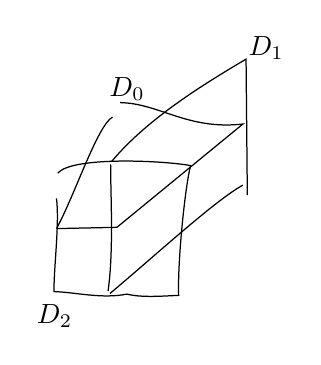
\begin{tikzpicture}[x=.80cm,y=.80cm,line width=.45pt]
\draw (0,1.48) .. controls (.05,1.1) and (-.04,.4) .. (-.04,0)
 .. controls (.30,-.01) and (.72,-.12) .. (1.12,-.04)
 .. controls (1.35,-.10) and (1.70,-.07) .. (1.94,-.06)
 .. controls (1.92,.46) and (2.04,1.66) .. (2.13,2)
 .. controls (1.70,2.08) and (.25,2.15) .. (.02,1.88);
\draw (.82,.01) .. controls (.91,.67) and (.86,1.5) .. (.86,2.02);
\draw (.88,2.07) .. controls (1.45,2.75) and (2.35,3.3) .. (3.01,3.69)
 -- (3.03,1.53);
\draw (.85,-.03) .. controls (1.52,.53) and (2.52,1.45) .. (2.96,1.69);
\draw (.00,1.00) .. controls (.28,1.5) and (.65,2.64) .. (.89,2.77);
\draw (.01,1.00) -- (.96,1.02) -- (2.96,2.66)
 .. controls (2.08,2.56) and (1.63,2.99) .. (1.01,3);
\node at (1.12,3.22) {$D_0$}; \node at (3.33,3.86) {$D_1$}; \node at (-.03,-.39) {$D_2$};
\end{tikzpicture}}

% lower group of signs written upside down
\diagram{\begin{tikzcd}[ampersand replacement=\&,column sep=small,row sep=small]
\& T\bigl(E_1,\ldots,E_n\bigr)^{\deleted{\unsure{\Phi}}} \& \deleted{\unsure{E}}\mathscr F\\
X \& \mathbb K\qquad\overset{\deleted{\unsure{n_1}}}{p_1}\qquad p_n \& {}\\
\& G_1\times\cdots\times G_{\unsure{m|n}} \& \unsure{\mathscr K|K|k}
\end{tikzcd}}
\scanpage{106}
\mspage{- IV- \handwritten{878} -}
% archive sheet number: 105
\uline{un point de} $Y$ .

Il résulte en effet de (17.4.1,(b'')) qu'une $Y$-section $s$ de $X$ est une
immersion ouverte , et comme $X$ est un $Y$-schéma , $s$ est aussi une \deleted{\unsure{imme}}
immersion fermée (\uline{I},5.4.7) ; il en résulte que $s$ est un isomorphisme de
$Y$ sur un sous-préschéma de $X$ induit sur une partie ouverte et fermée de
$X$ , et comme \deleted{\unsure{$X$|$Y$}} $s(Y)$ est connexe , cést nécessairement une composante
connexe de $X$ . Le reste de la proposition est immédiat .

\handwritten{[}\uline{Proposition} (17.4.10) .- \uline{Soient} $g:Y\to S$ , $h:X\to S$ \uline{deux morphismes localement de présentation finie . Pour qu'un} $S$-\uline{morphisme} $f:X\to Y$ \uline{soit non ramifié
il faut et il suffit que pour tout} $s\in S$ , \uline{le morphisme} $f_s:h^{-1}(s)\to g^{-1}(s)$
\uline{déduit de $f$ par le} \deleted{\unsure{morph|chang}} \uline{changement de base} $\operatorname{Spec}(\kappa(s))\to S$ , \uline{soit non ramifié}.

Cela résulte aussitôt du fait que pour un morphisme localement de présentation finie , le fait d'être non ramifié est une propriété des \uline{fibres} de ce
morphisme\inserted{ (17.4.1,d))}, et \inserted{\handwritten{de ce}} que pour tout $y\in Y$ , on a $f^{-1}(y)=f_s^{-1}(y)$ si $s=g(y)$ .\handwritten{]}

\uline{17.5. Caractérisations des morphismes lisses} .

\uline{Théorème} (17.5.1) .- \uline{Soient} $f:X\to Y$ \uline{un morphisme localement de présentation finie , $x$ un point de} $X$ , $y=f(x)$ . \uline{Les conditions suivantes sont équivalentes} :

a) \uline{$f$ est lisse au point $x$} .

b) \uline{$f$ est plat au point $x$ et le} $\kappa(y)$-\uline{préschéma} $f^{-1}(y)$ \uline{est lisse sur} $\kappa(y)$
\uline{au point $x$} .

b') \uline{$f$ est régulier au point $x$} (6.8.1) .

c) \uline{L'anneau} $O_{X,x}$ \uline{est une} $O_{Y,y}$-\uline{algèbre formellement lisse pour les topologies discrètes} .

On peut se borner au cas où $Y=\operatorname{Spec}(A)$ , \deleted{\unsure{$X=\operatorname{Spec}(B)$}} $X=\operatorname{Spec}(C)$ , où $C=B/\underline J$
$B=A[T_1,..,T_n]$ étant une algèbre de polynômes et $\underline J$ un idéal de $B$ \uline{de type fini} . L'équivalence de a) et c) résulte alors de (\uline{0},22.6.4)\inserted{ \handwritten{a)$\Leftrightarrow$c)}} . D'autre
part , comme $f^{-1}(y)$ est un $\kappa(y)$-préschéma localement \deleted{noethérien}\inserted{\handwritten{de type fini}} , l'équivalence de b) et b') résulte de (6.8.6)\inserted{ \handwritten{a)$\Leftrightarrow$b)}} . Reste à voir que a) et b)
sont équivalentes .
\margin{\handwritten{Attention à l'\unsure{ambiguïté|ambiguité} dans ``lisse'' !}}
\scanpage{107}
% archive sheet number: 106
\figure{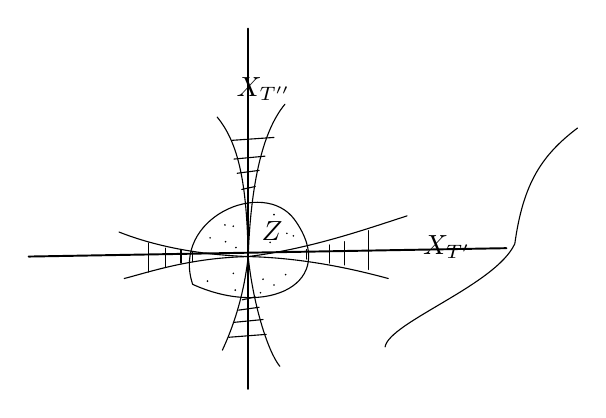
\begin{tikzpicture}[x=.82cm,y=.82cm,line cap=round]
\draw[line width=.7pt] (-3.40,0)--(4.00,.13);
\draw[line width=.7pt] (0,-2.05)--(0,3.53);
\draw (0,0) .. controls (-.02,1.14) and (-.15,1.76) .. (-.48,2.16);
\draw (0,0) .. controls (.04,1.12) and (.22,1.94) .. (.57,2.36);
\draw (0,0) .. controls (-.07,-.64) and (-.25,-1.13) .. (-.40,-1.45);
\draw (0,0) .. controls (.07,-.69) and (.29,-1.45) .. (.49,-1.70);
\draw (0,0) .. controls (-.80,.03) and (-1.47,.17) .. (-2.00,.38);
\draw (0,0) .. controls (-.90,-.02) and (-1.53,-.24) .. (-1.92,-.34);
\draw (0,0) .. controls (.96,.12) and (1.81,.42) .. (2.46,.63);
\draw (0,0) .. controls (.85,-.02) and (1.62,-.19) .. (2.17,-.34);
\draw (-.86,-.43) .. controls (-1.20,.60) and (.24,1.23) .. (.72,.57)
 .. controls (1.42,-.41) and (.30,-.96) .. (-.86,-.43);
\foreach \x/\a/\b in {-1.54/-.24/.21,-1.28/-.17/.13,-1.04/-.10/.10,-.86/-.08/.07,.91/-.04/.11,1.26/-.10/.18,1.49/-.13/.23,1.86/-.20/.40}
{\draw (\x,\a)--(\x,\b);}
\foreach \y/\a/\b in {1.80/-.25/.40,1.51/-.22/.26,1.29/-.17/.17,1.04/-.10/.11,-.67/-.09/.11,-.83/-.15/.17,-1.02/-.23/.23,-1.25/-.30/.28}
{\draw (\a,\y)--(\b,\y+.045);}
\foreach \x/\y in {-.59/.29,-.36/.49,-.23/.47,-.35/.23,-.19/.14,.40/.65,.60/.36,.70/.32,.34/.22,-.63/-.38,-.23/-.26,-.20/-.52,.23/-.35,.40/-.44,.58/-.28,.19/-.56}{\fill (\x,\y) circle (.014);}
\draw[thin] (2.12,-1.40) .. controls (2.18,-1.02) and (3.84,-.44) .. (4.13,.20) .. controls (4.26,1.15) and (4.56,1.58) .. (5.10,1.99);
\node at (.37,.39){$Z$};\node at (.24,2.60){$X_{T''}$};\node at (3.08,.15){$X_{T'}$};
\end{tikzpicture}}

\diagram{\begin{tikzcd}[ampersand replacement=\&,column sep=small,row sep=small]
\& \& \& \deleted{\unsure{*}} \& {}\\
\& \widehat{\mathbb Z}=\pi_1(Z')\arrow[dl]\arrow[drrr] \& \& \pi_1(Z'')=\widetilde{\mathbb Z}\arrow[dl]\arrow[dr] \& {}\\
\pi_1(X_{T'})\arrow[drr] \& \& \pi_1(X_{T''})\arrow[d] \& \& \pi_1(Z)=\widehat{\mathbb Z}^{\,2}\arrow[dll]\\
\& \& \pi_1(X_T) \& \& {}
\end{tikzcd}}

$Z=\operatorname{Spec}\widehat{\underline{\mathrm O}_{X,a}}$\inserted{$A$}

$X_{T'}\cap X_{T''}=\varnothing$

$X_{T'}\cap Z_{\deleted{\unsure{T'}}}=Z'=\widehat A_{p'}$ correspond au corps
résiduel $k(p')={}$ corps local en $a$ de $T'_0$

$X_{T''}\cap Z=Z''=\widehat A_{p''}$ correspond au corps
résiduel $k(p'')={}$ corps local en $a$ de $T''_0$

On doit prouver un \uline{\unsure{th|thm|th.} de descente}
de nature essentiellement locale

$+$ déterminer certains hom. canoniques

\[
-\quad-\quad-
\]

\diagram{\begin{tikzcd}[ampersand replacement=\&,row sep=tiny]
\deleted{\unsure{A'}}\arrow[d,no head,bend right=12]\\ A\arrow[d]\\ B
\end{tikzcd}}
\scanpage{108}
% archive sheet number: 107
% Mirrored typescript shows through the sheet.
\[
P=QQ' \qquad QR+Q'R'=1 \qquad (P)=(Q)(Q')=(Q)\cap(Q')
\]
\[
 A[t]/(P)\longrightarrow A[t]/(Q)\times A[t]/(Q')
\]
\margin{car $s\in(Q)$, $s\in(Q')$\\
$\Longrightarrow s=Q'sR'+QsR\in(QQ')$}

injectif car $(\deleted{\unsure{Q}}P)=(Q)\cap(Q')$

Surjectif car par Nakayama on est ramené au cas

$A[t]$

\uline{Lemme} Soient $Q,Q'\in A$ \unsure{parties|idéaux} \uline{\unsure{étrangères|étrangers}}.

Alors $A/(QQ')\longrightarrow A/Q\times A/Q'$ est un isom.

En effet, (i) $(Q)\cap(Q')=Q.Q'$

car $\underline Q\cap\underline Q'=\underline Q\cap\underline Q'(\underline Q+\underline Q')\subset
\underline Q'\,\underline Q+QQ'=QQ'$

(ii) $\underline Q+\underline Q'=A$ par hypothèse ; on peut pour
\[
\begin{aligned}
 x\in A,\;y\in A\quad\Longrightarrow\quad&\exists\,\unsure{b|a}\in Q\quad\text{qui est }\equiv y\quad(Q')\\
 &\exists\,\unsure{a|b}\in Q'\quad\text{qui est }\equiv x\quad(Q).
\end{aligned}
\]
donc $a+b\equiv\begin{cases}x&(Q)\\ y&(Q')\end{cases}$

\diagram{\begin{tikzcd}[ampersand replacement=\&,column sep=small,row sep=small]
 A/Q.Q'\arrow[r] \& A/Q\mathbin{\unsure{\to|-}} A/Q' \& \text{surjectif}\ \deleted{\unsure{\text{tel}}}\arrow[d,Leftrightarrow] \& {}\\
 \& \& \text{bijectif}\arrow[d,Leftrightarrow] \& {}\\
 \& \& Q+Q'=A\arrow[r,Rightarrow] \& QQ'=Q\cap Q'
\end{tikzcd}}
\scanpage{109}
% archive sheet number: 108
\begin{center}Ad majorem fonctori gloriam\end{center}

J'apprends que Grothendieck n'est plus membre de Bourbaki. Je le regrette
beaucoup, ainsi que les circonstances qui ont amené cette décision.

Il est bien entendu admis que Grothendieck n'aime pas la taquinerie ni le
canular, tous deux chers à Bourbaki. Mais on se rode, et il était en bonne
voie dans cette direction. D'autres y ont passé avant lui. De toute façon,
ceci n'était qu'un côté secondaire de la question. Ce qui importait, c'est
une opposition systématique, plus ou moins explicité selon les uns ou les
autres, contre son point de vue mathématique, ou plutôt son emploie par
Bourbaki.

Or, comme l'a très bien remarqué Kaplanski dans sa dernière review,
Bourbaki n'est plus le youth impétueux qu'il était il y a vingt ans, mais une
fixture moyenne-ageuse, ce qui est fort regrettable, mais malheureusement vrai.

C'est un scandale que Bourbaki, non seulement ne soit pas à la tête du
mouvement fonctoriel, mais encore n'y soit même pas à la queue. Si Bourbaki
tient à rester ce qu'il a voulu être, il est temps qu'il se réveille. Si
certains membres fondateurs (e.g. Weil) désirent revenir sur leur décision de
ne pas influencer Bourbaki dans la direction qu'il désire prendre, qu'ils le
disent explicitement. A mon avis, c'est contraire aux habitudes de Bourbaki
de trainer dans l'équivoque.

Comme suggestion pratique, je commence par proposer que Bourbaki adopte
le livre de Grothendieck sur les catégories, ou toute autre variante, par
exemple un fascicule de résultats extrait dudit livre.

Si Bourbaki refuse, non pas de se mettre dans le nouveau mouvement, mais
d'en prendre la tête, alors les traités visant à la rédaction des éléments de
mathématiques (et pas seulement à ceux de la géométrie algébrique) seront
rédigés par d'autres, qui s'inspireront non pas de l'esprit de Bourbaki 1960,
mais de son esprit 1936. Ce serait dommage.

\begin{center}-:-:-:-\end{center}

Je prends l'occasion pour indiquer une liste de questions catégoriques
\scanpage{110}
% archive sheet number: 109
a) Donnons nous un idéal $R\subset B$. Alors

Décomposition de $\deleted{\unsure{A}}B/R$ en produit de deux anneaux

$\simeq$ Donnée de deux idéaux $J,J'$ de $A$ tels que
\[
JJ'=R,\quad J+J'=A\qquad [\text{Car }J+J'=A\Rightarrow JJ'=J\cap J']
\]

b) Supposons $B=A[T]$, \inserted{\deleted{$A$ \unsure{local donc}} $A$ connexe} $R=(P)$, $P$ polynôme
\uline{unitaire}, Alors tte décomposition de $R$ en
produit de deux idéaux $J,J'$ tels que $J+J'=B$,
est uniquement de la forme $(\deleted{\unsure{R}}P)=(Q)(Q')$, où
$Q,Q'$ sont des polynômes \uline{unitaires} tels que
$P=QQ'$.

Si elle est \unsure{donnée|dominée} par une telle déc,
alors $P$ est unique à une unité près,
et étant supposé \unsure{unifaire|unitaire} est unique
\deleted{[N.B. tout} [petite vérification \ldots.]. \deleted{On
\unsure{prouvera que}} De l'unicité résulte que
l'on peut supposer $\operatorname{Spec} A$ \uline{local}. Alors pour
l'existence, on note que c'est vrai sur les
\scanpage{111}
\deleted{\unsure{exaltation} par contre ne pourrait que m'inquiéter sérieusement}

\[
\begin{aligned}
&A\ \text{anneau local }\deleted{\unsure{\text{régulier}}} && \widehat A\ \text{son complété}\\
&X=\operatorname{Spec}(A) && \widehat X\\
&D.\ \text{partie fermée} && \widehat D
\end{aligned}
\]

\figure{\begin{tikzpicture}[x=.0072cm,y=-.0072cm,line cap=round,line join=round]
\draw[thin] (65,28) .. controls (30,4) and (450,15) .. (950,-12) .. controls (1110,-24) and (1350,-50) .. (1435,-30) .. controls (1507,-12) and (1508,155) .. (1437,229) .. controls (1370,304) and (1250,247) .. (1134,361) .. controls (1060,436) and (984,576) .. (1076,600) .. controls (1140,621) and (1328,566) .. (1375,575) .. controls (1421,575) and (1369,654) .. (1435,752) -- (1591,961);
\draw (75,405) .. controls (75,574) and (88,625) .. (214,650) .. controls (302,665) and (417,650) .. (481,673);
\draw (105,120)--(177,48)--(175,101) (201,45) .. controls (254,64) and (277,39) .. (303,48) (314,61)--(310,209)--(225,258);
\draw (95,133)--(238,129)--(237,244) (93,139)--(89,251) .. controls (147,254) and (190,264) .. (218,252);
\draw (96,200)--(235,193) (243,201)--(306,198) (107,242)--(154,206) (203,77) .. controls (246,68) and (225,116) .. (266,113);
\draw[densely dotted] (100,171).. controls (126,142) and (165,104)..(237,110);
\draw (91,167).. controls (170,127) and (211,175)..(235,239) (91,195)--(145,138) (232,243)--(312,171)--(281,132) (250,251)--(292,216);
\draw (216,185)..controls (230,173) and (223,163)..(223,153);
\fill (223,152) circle (4); \fill (237,110) circle (3);
\draw (478,109)--(567,27) (580,22) .. controls (640,17) and (686,25) .. (736,26)--(731,191)--(655,257);
\draw (492,100) .. controls (568,95) and (630,113) .. (655,101) (493,106)--(487,252) (492,252) .. controls (542,250) and (594,267) .. (645,259)--(664,115)--(736,27);
\draw[dashed] (575,32)--(565,188)--(491,252) (568,188)--(729,190);
\draw[thick] (491,194)--(654,190)--(730,119)--(572,119)--cycle;
\draw (606,101).. controls (614,116) and (617,138) .. (612,159) (616,157).. controls (638,144) and (661,165)..(692,144);
\fill (612,159) circle (10);
\draw[thick] (888,121).. controls (916,105) and (922,68) .. (930,48) .. controls (959,57) and (994,50) .. (1022,47) .. controls (1014,75) and (999,107) .. (980,130) .. controls (954,137) and (918,130) .. (888,121);
\fill (961,89) circle (10);
\node at (1116,218) {$\times$};
\node at (1262,147) {$\deleted{\unsure{Z\quad fX_{i}}}$};
\node at (331,400) {$\widehat Y\unsure{\to|\times|\hookrightarrow}\widehat Z$};
\node at (670,400) {$\widehat Y\times_{\widehat S}\widehat Z$};
\node at (986,401) {\deleted{\illegible{1}}};
\node at (312,513) {$Y\times Z$};
\node[anchor=west] at (475,515) {composante connexe};
\node at (470,580) {\begin{tikzcd}[ampersand replacement=\&,row sep=1.2em] H\arrow[d]\\ Y\times Z\end{tikzcd}};
\draw (23,724) .. controls (80,707) and (360,675) .. (512,684) .. controls (586,697) and (537,898) .. (552,1012);
\draw (63,1012) .. controls (132,1014) and (206,1018) .. (189,961) .. controls (176,907) and (132,834) .. (211,798) .. controls (278,765) and (376,791) .. (403,815) .. controls (464,875) and (400,937) .. (371,990) .. controls (352,1032) and (398,1040) .. (423,1031) -- (506,1032);
\draw (578,684) .. controls (672,633) and (645,984) .. (682,1192);
\draw[thin] (695,673) .. controls (758,618) and (830,690) .. (783,755) .. controls (704,876) and (628,740) .. (695,673);
\node at (1297,870) {\begin{tikzcd}[ampersand replacement=\&,column sep=.85em,row sep=1.1em]
 S \& \widehat S\arrow[l] \& {}\\
 X\arrow[u] \& \widehat X\arrow[u]\arrow[l] \& {}\\
 \deleted{\unsure{Y}}\, A\arrow[u]\arrow[r,dash] \& A'\arrow[u]\arrow[r,dash] \& \widehat A=\widehat{A'} 
 \end{tikzcd}};
\draw[very thick] (1410,1054)--(1465,1112) (1560,1035)--(1621,1090);
\draw (711,1128) .. controls (796,1098) and (873,1082) .. (935,1092) (803,1050)--(868,1132) (848,1036).. controls (830,1100) and (824,1155)..(829,1190);
\draw (965,981)--(1008,1062) (1012,975)..controls (981,1011) and (968,1076)..(970,1127);
\draw (887,1170)--(921,1272) (922,1155)..controls (891,1206) and (903,1294)..(905,1317);
\draw (1082,1045)..controls (1070,1130) and (1108,1211)..(1134,1280) (1011,1251)..controls (1061,1184) and (1114,1159)..(1174,1140);
\fill (1103,1176) circle (5);
\draw (1218,1082)--(1254,1208) (1252,1084).. controls (1220,1177) and (1227,1216)..(1239,1264);
\draw (1321,1183)--(1395,1177) (1321,1217)--(1361,1170)--(1394,1160) (1345,1140)..controls (1344,1182) and (1363,1200)..(1381,1215);
\end{tikzpicture}}
% crop-candidate: scan 111
% archive sheet number: 110
